\begin{section}{Implementation and Power Spectra}
  \label{sec:simulation}
  We use the \textsc{CUBEP$^3$M} code \cite{bib:Harnois2013} to run
  140 simulations with a box size of 600 Mpc/h and $512^3$ particles.
  The initial conditions are computed using the transfer function
  given by CAMB \cite{bib:Lewis2000} and then propagating the power
  back to $z=100$ with a linear growth factor.  The Zel'dovich
  approximation is used to calculate the displacement and velocity
  fields of the particles.  For these simulations, we use cosmological
  parameters $\Omega_M=0.321$, $\Omega_{\Lambda}=1.0-\Omega_m$,
  $h=0.67$, $\sigma_8=0.83$, and $n_s=0.96$.  Different random seeds
  are used to produce the initial conditions for different simulations
  so that they are independent of each other.

  \begin{figure}[h]
    \centering
    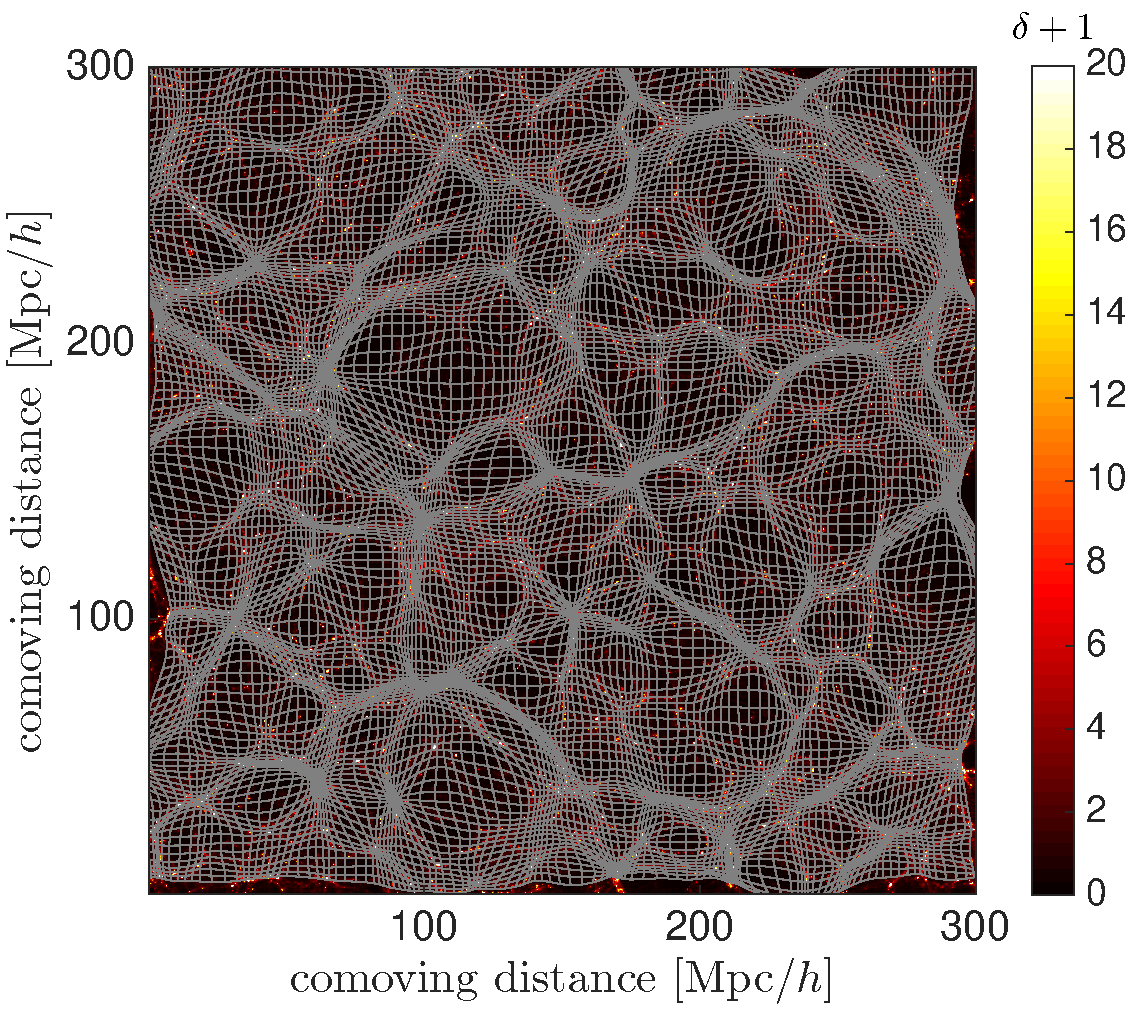
\includegraphics[width=0.45\textwidth]{fig1.pdf}
    \caption{ The 2-D projection of one layer of the deformed grid of a sample
      $N$-body simulation is shown as curved white lines.  The
      density fluctuation on the grid, $\delta\rho/\bar{\rho}$, is shown
      underneath.}
    \label{fig:simandrec}
 \end{figure}

  We use Voronoi tessellation method to estimate the density
  contrast $\delta_S=\delta\rho/\rho-1$ from the particles, and then
  apply the MM reconstruction to these fields with a resolution of
  $512^3$ cells.  The reconstruction code solves the dispacement potentials 
  iteratively until the root mean square (rms) drops 
  to 0.20 (typically from $\sim 7.5$). For different simulation samples, a different number of iterations are required to get 
  the results of the same rms. In total, 130 simulations converged within 2000 iterations.
  %We finally pick 130 simulation samples to do the remaining calculation, 
  %each among which gives a final rms of 0.20
  %through running the reconstruction code for no more than 2000 time steps. 
  A 2-D projection of one layer of the deformed grids and the
  original density field on the grids are given in Fig.~\ref{fig:simandrec}.  As
  expected, there is no grid crossing after reconstruction.
 
 The cross power spectrum, $P_{ab}(k)$, is defined as
 \begin{align}
   \langle \delta_a(\bm{k})\delta_b(\bm{k'}) \rangle =
   (2\pi)^3 P_{ab}(k) \delta_{3D}(\bm{k}-\bm{k'}),
 \end{align}
 where $\delta_{a}$ and $\delta_{b}$ are any density contrasts and
 $\delta_{3D}$ is the three-dimensional Dirac delta function. We typically consider instead
 the dimensionless power spectrum, $\Delta_{ab}^2(k)$, defined as
 \begin{align}
   \Delta_{ab}^2(k) \equiv \frac{k^3 P_{ab}(k)}{2\pi ^2}.
 \end{align}
 In the left panel of Fig.~\ref{fig:cp}, we show the matter auto power
 spectrum ($a=b$) of linear theory density fields ($\delta_L$), from
 the simulation results ($\delta_S$) and after reconstruction
 ($\delta_R=-\nabla^2\phi$).  For the simulation
 results, we use the average value of all 130 simulations and show
 the $1\sigma$ standard deviation as error bars.  To determine the correlation
 between fields, we compute the cross correlation coefficient
 $r_{ab}(k) = P_{ab}/\sqrt{P_{aa}P_{bb}}$.  In the right panel of
 Fig.~\ref{fig:cp}, we show $r_{SL}$ and $r_{RL}$.  We see that the
 reconstructed field is much more highly correlated with the linear
 field than the simulation field is.  For comparison, we also plot the 
 correlation coefficient of $\delta_E$ 
 and $\delta_L$ from \citet{bib:Yu2016}, 
 where $\delta_E(\bs{q})= - \nabla_q \cdot \bs{\Psi}(\bs{q})$ is the 
 negative divergence of the real non-linear displacement computed by tracking particle positions. 
 Ideally, the MM algorithm aims to get the cross correlation $r_{RL}$ close to $r_{EL}$. 
 Even though $r_{RL}$ decreases from $r_{EL}$ in the non-linear regime, due to the fact that the MM reconstruction 
 cannot recover the cell-crossing and vorticity present on these scales, we find that linear modes are recovered successfully on scales $k\simeq 0.05 - 0.3$ h/Mpc.
 Specifically, the scale at which $r(k)=1/2$ increases from $k\simeq 0.2$ h/Mpc to
 $0.8$ h/Mpc after reconstruction.  In comparison with the results of \citet{bib:ZhuH2016},
 we find the correlation coefficient falls off at slightly lower
 wavenumbers, which we believe is from using fewer particles per simulation.

  \begin{figure*}
    \centering
    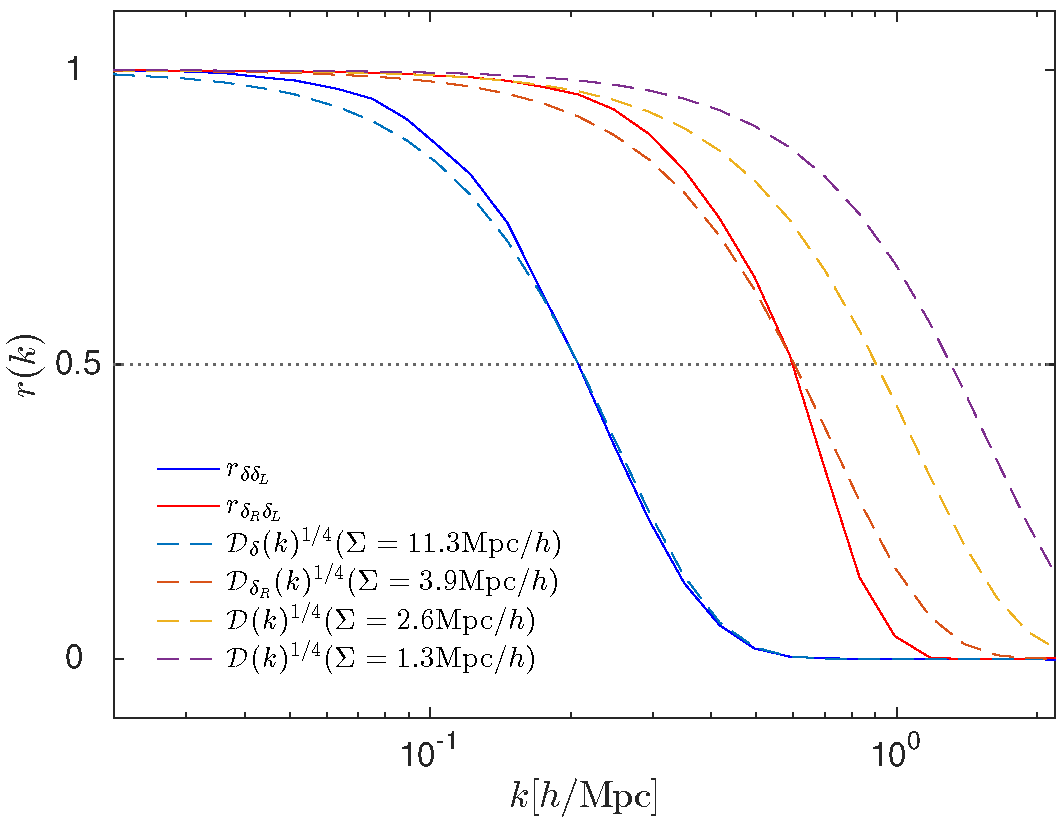
\includegraphics[width=0.5\textwidth]{fig2a.pdf}
    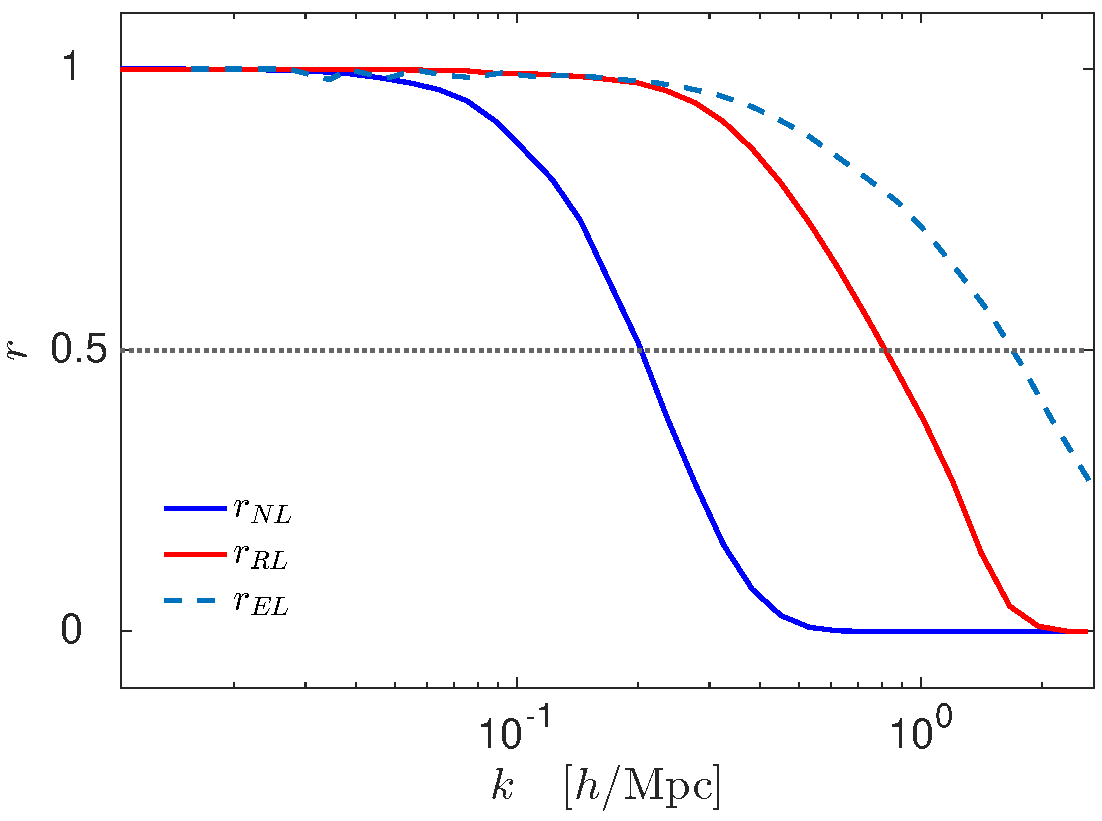
\includegraphics[width=0.49\textwidth]{fig2b.pdf}
    \caption{{\it Left.} The dimensionless power spectrum computed via
      linear theory (black), the mean value of 130 $N$-body
      simulations with $1\sigma$ error bars (blue), and reconstruction
      of the simulations (red).  {\it Right.} The cross correlation
      function between simulation and linear densities $r_{SL}$ (blue),
      MM reconstructed and linear densities $r_{RL}$ (red), and E-mode reconstruction $r_{EL}$ (dash
      blue) from \citet{bib:Yu2016}.}
    \label{fig:cp}
  \end{figure*}


\end{section}

